\documentclass[../main.tex]{subfiles}
\begin{document}
\paragraph{Simulation 2}\label{par:sim_2}

\begin{equation}\label{eq:sim_2_shift}
        g(s) \in \mathbb{P}_{4}[s]\,,\quad\{c_{1}=-1.6,\, c_{2}=-2,\, c_{3}=2.6,\, c_{4}=2\}\,.
\end{equation}

The critical points of $\newprime{g}$ are $t_{1} = ? \;\Rightarrow\;\newprime{f}(t_{1}) = 0.33796$ and $t_{2} = ? \;\Rightarrow\;\newprime{f}(t_{2}) = -1.6155$.
As such we have

\begin{equation*}
        L = \sup\,(-\infty,1.61155] = \inf\,[1.61155,+\infty)\,.
\end{equation*}

\begin{figure}[H]
    \centering 
    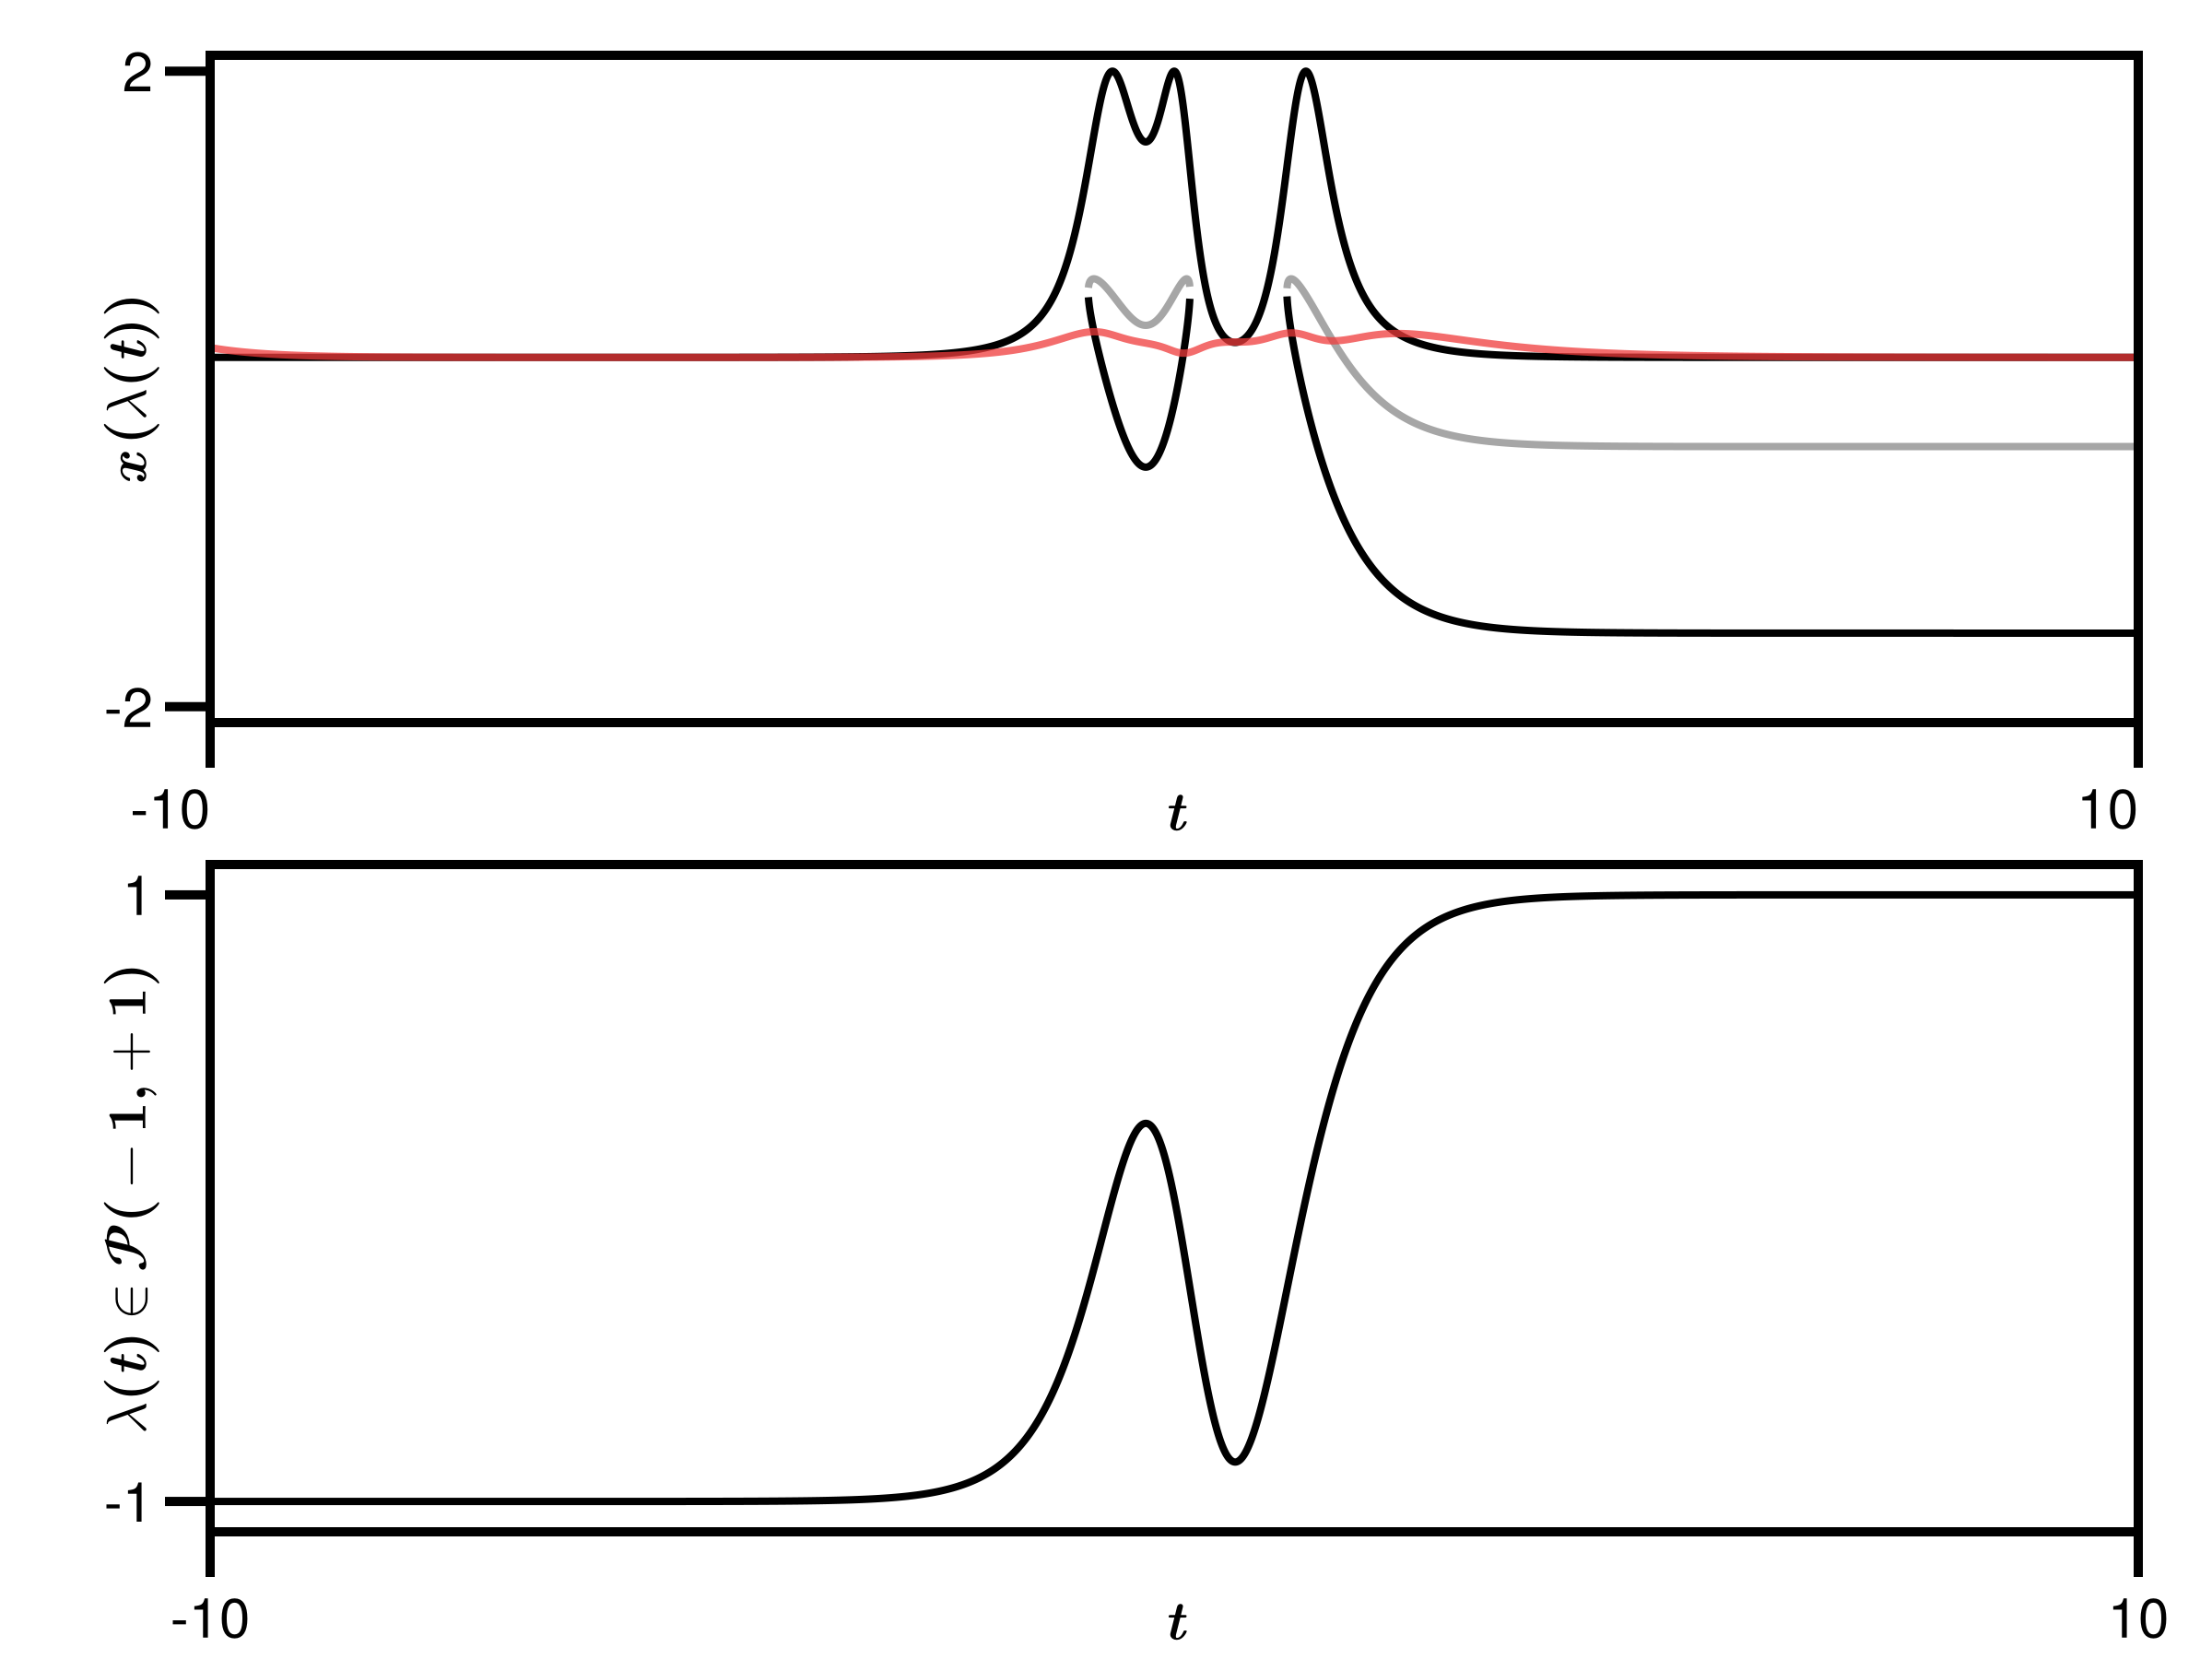
\includegraphics[keepaspectratio, width=\textwidth]{../figures/sim_2.png}
    \caption{Solution of \eqref{eq:dyn_sys} (top) with the parameter shift \eqref{eq:sim_2_shift} (bottom). No R-tipping.}
    \label{fig:sim_2}
\end{figure}

\end{document}
